\chapter{Metodología}
Para la implementación del producto se utilizará la metodología Desarrollo Rápido de Aplicaciones (Rapid Application Development –RAD- en inglés) que se basa en el desarrollo de prototipos funcionales, los cuales sirven para que el cliente de un feedback y así se desarrolle en conjunto y aproximarse mejor a lo que el cliente desea.

RAD está conformado por varias fases, las cuales son:
\begin{itemize}
\item Análisis y diseño rápido: se hace un análisis de los requerimientos y se realiza un diseño a modo de borrador basado en el análisis, el cual es tomado en cuenta pero no es de gran importancia ya que el producto final es el resultado de varias iteraciones hechas con prototipos funcionales entregados.
\item Prototipado (construir, demostrar y refinar): se realizan prototipos funcionales basados en las necesidades de los usuarios, los requerimientos y en el diseño hecho anteriormente. Estos prototipos sirven para demostrar las capacidades de la aplicación paso a paso y obtener una respuesta por parte de los usuarios.
\item Pruebas: se realizan pruebas unitarias del código que se tiene para asegurar el correcto funcionamiento.
\item Implementación: se elabora un producto final, el cual está basado y formado por los diferentes prototipos utilizados durante el proceso de desarrollo.
\end{itemize}
\begin{figure}
\centering
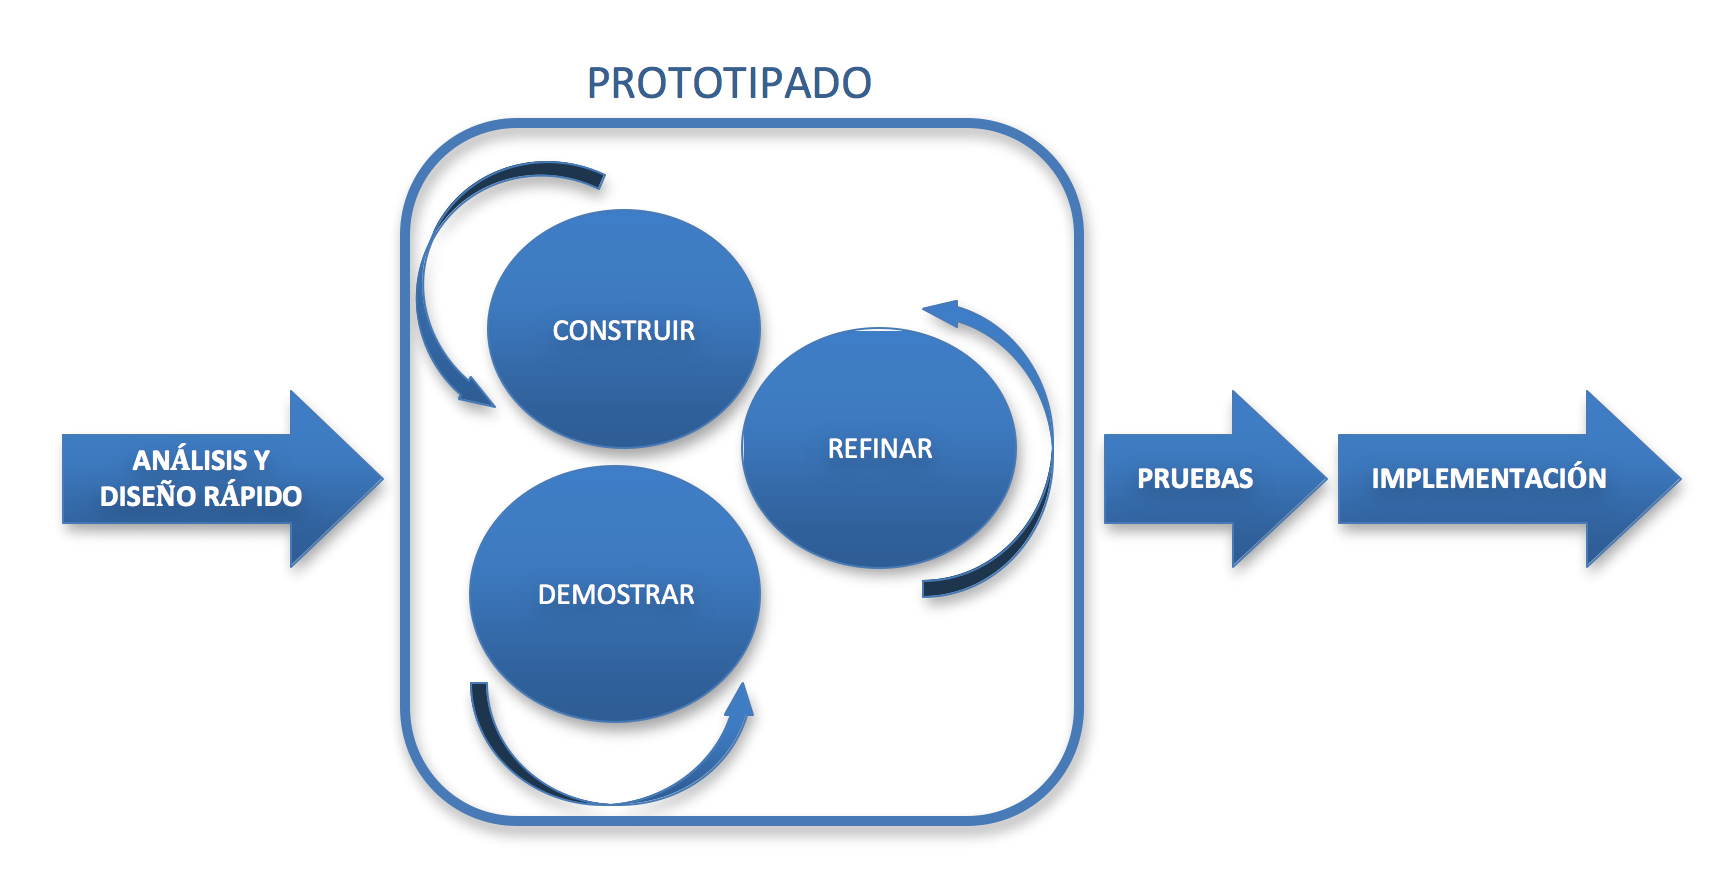
\includegraphics[scale=0.5]{imagenes/metodologia}
\caption{Metodología de desarrollo RAD}
\label{fig:metodologia}
\end{figure}
